\newpage
\section{The luminosity spectra of the ILC250 beam parameter sets}
\label{sec:Envelopes}
The processes, in which the beamstrahlung from beam-beam interactions produces secondary \Pep \Pem pairs, were simulated with \guineapig~\cite{Schulte:1997nga}.
\guineapig is a Monte Carlo (MC) background event generator comparable to CAIN~\cite{CAIN}, which was used for the ILC250 background studies presented at AWLC17~\cite{AWLC_Jeans}.\\
Using the beam particle distributions generated by \guineapig, the luminosity spectra of the ILC250 stage parameters can be plotted as shown in Figure~\ref{fig:Lumi_Spectra}.
\begin{figure}[h]
\centering
\begin{subfigure}[t]{0.49\textwidth}
\centering
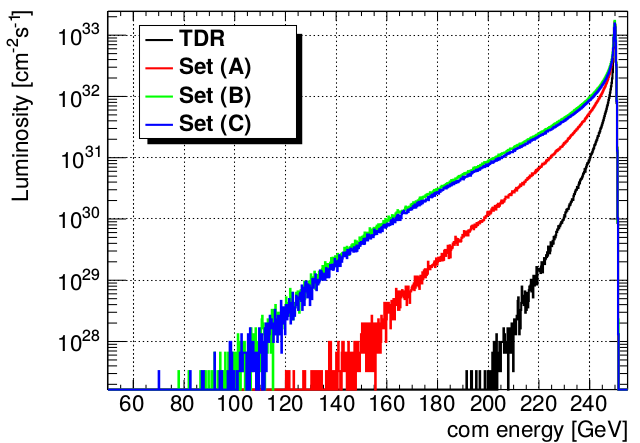
\includegraphics[width=\textwidth]{figures/Lumi_Spectrum.png}
\caption{}
\end{subfigure}
\hspace*{0.08cm}
\begin{subfigure}[t]{0.49\textwidth}
\centering
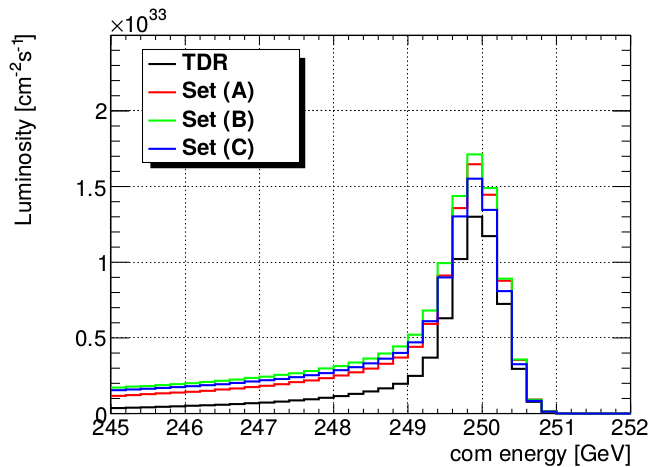
\includegraphics[width=1.02\textwidth]{figures/Lumi_Spectrum_zoom.png}
\caption{}
\end{subfigure}
\caption{\textit{Luminosity spectra generated with \guineapig, using the ILC250 parameter sets listed in Table~\ref{tab:Parameters}.
Figure (b) shows the spectra zoomed in at around \SI{250}{\GeV}.}}
\label{fig:Lumi_Spectra}
\end{figure}
\\Comparing the total luminosity resulting from the spectra in Figure~\ref{fig:Lumi_Spectra}, the expected rise in the luminosity due to the reduction of the horizontal beam emittance and the beta function is demonstrated.
\\The value for the TDR set (\SI{8.26e33}{\per\centi\meter\squared\per\second}) confirms the calculations of the luminosity done for the Change Request CR-005, which states a value of \SI{8.2e33}{\per\centi\meter\squared\per\second}~\cite{CR-005}.
The new official beam parameters of set (A) produce a luminosity of \SI{1.62e34}{\per\centi\meter\squared\per\second}, which is an increase of about \SI{97}{\percent}.
\begin{table}[h]
\centering
\begin{tabularx}{0.4\textwidth}{cc}
\hline\hline
\textbf{Set}  & Luminosity [\si{\per\centi\meter\squared\per\second}]\\
\hline
\cline{1-2}
\hline
 TDR & \num{8.26e33}\\
 \rowcolor{Gray}
 (A) & \num{1.62e34}\\
 (B) & \num{2.38e34}\\
 (C) & \num{2.15e34}\\
\hline\hline
\end{tabularx}
\caption{\textit{The total luminosities resulting from the luminosity spectra generated with \guineapig for the different ILC250 beam parameter sets.}}
\label{tab:Luminosity}
\end{table}